\documentclass[12pt]{beamer}
\usepackage[utf8]{vietnam}
\usepackage{lmodern}
\usepackage{animate}
\usepackage{wrapfig}
\usetheme{metropolis}

\begin{document}
	\author{Đặng Quang Anh - Cao Việt Tùng}
	\title{TABU SEARCH}
	\date{Tháng 6 2021}
	%\subtitle{}
	%\logo{}
	%\institute{}
	%\date{}
	%\subject{}
	%\setbeamercovered{transparent}
	%\setbeamertemplate{navigation symbols}{}
	\maketitle
	
	\frame<beamer>{
		\frametitle{Outline}
		\tableofcontents
	}

	\section{Search Space and Neighbor Structure}
	\begin{frame}
		\frametitle{Search Space and Neighbor Structure}
		\begin{itemize}
			\item Không gian tìm kiếm: Là khoảng không gian của tất cả các giải pháp có thể xem xét (ghé thăm) trong quá trình tìm kiếm.
			\item Cấu trúc vùng lân cận: Là một tập con của Không gian tìm kiếm định nghĩa bởi\\
					$N(S) = \{ $giải pháp thu được bằng cách áp dụng một biến đổi cục bộ duy nhất cho S$ \}$
		\end{itemize}
	\end{frame}

	\begin{frame}
		\frametitle{Search Space and Neighbor Structure}
		Ví dụ:\\
		Một người giao hàng cần đi giao hàng tại 5 thành phố. Xuất phát từ một thành phố bất kì, đi qua các thành phố khác  và trở về thành phố ban đầu, mỗi thành phố chỉ đến một lần. Hãy tìm một đường đi thỏa mãn điều kiện trên sao cho tổng độ dài là nhỏ nhất.\\
		\begin{itemize}
			\item Không gian tìm kiếm là tập hợp tất cả các cách đi khả thi của người bán hàng
			\item Với một cách đi S của người bán hàng (giả sử là a-b-c-d-e) thì bằng cách đổi chỗ 2 thành phố bất kì trong cách đi trên ta thu được một cách đi (ví dụ a-c-b-d-e) và đó là một lân cận của S.
		\end{itemize}
	\end{frame}
	
	\section{Tabus}
	\begin{frame}
		\frametitle{Hill Climbing}
		Giải thuật leo đồi (Hill Climbing): Ở mỗi lần lặp, tìm giải pháp tốt hơn giải pháp hiện tại trong vùng lân cận (Neighbor Structure), nếu không có thì thuật toán dừng lại. Điều đó dẫn đến thuật toán có thể bị kẹt lại tối ưu cục bộ.\\
		Ví dụ:\\
		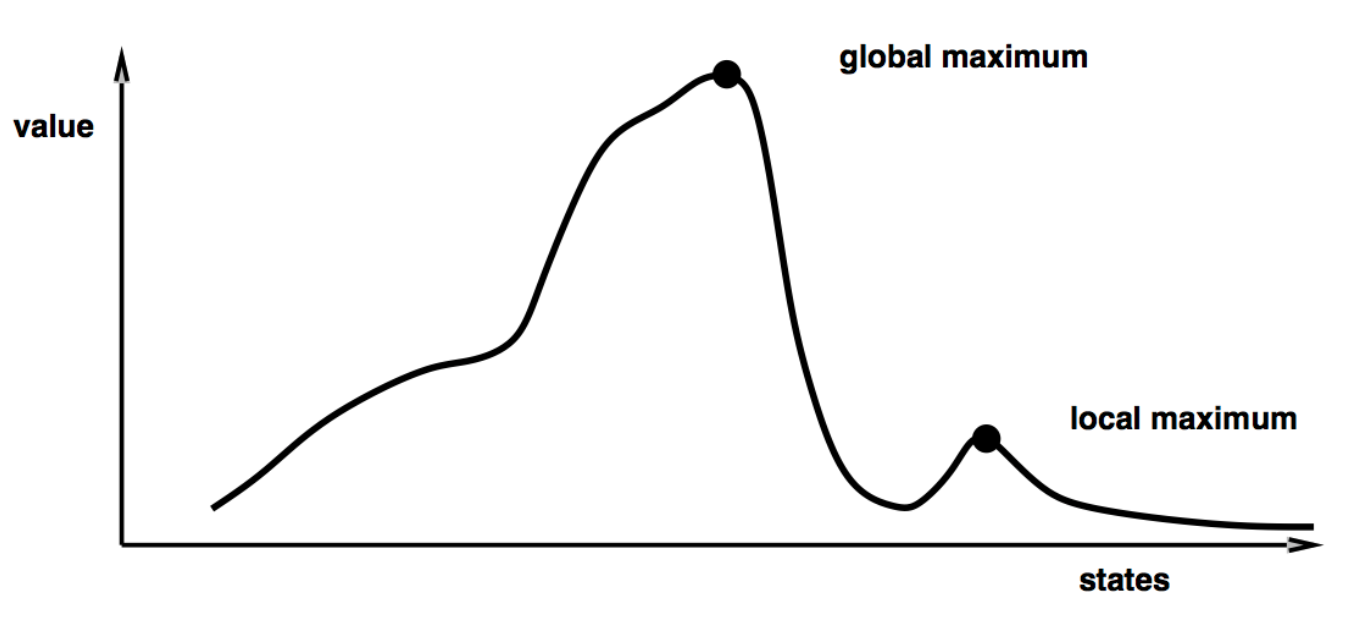
\includegraphics[scale=0.4]{HillClimbing.png}\\
	\end{frame}

	\begin{frame}
		\frametitle{Tabus}
		Tabu Search cho phép di chuyển khỏi tối ưu cục bộ bằng các bước đi không cải thiện.\\
		Khi đó, có khả năng rằng thuật toán sẽ đi ngược lại những bước đã đi qua và trở về điểm xuất phát. Như vậy ta cần làm gì đó để ngăn không cho điều này xảy ra.\\
		Ta thực hiện việc này bằng cách sử dụng Tabus.
	\end{frame}

	\begin{frame}
		\frametitle{Tabus}
%		Một bước đi được gọi là Tabu nếu nó đã được đi trong một số lần tìm kiếm trước đó.\\
		Tabus được lưu trữ trong bộ nhớ ngắn hạn của cuộc tìm kiếm (tabu list)\\
		Ví dụ:\\
		Như ở ví dụ trước để có được cách đi a-c-b-d-e từ a-b-c-d-e ta đã đổi chỗ b từ vị trí 2 đến 3 nên tabus có thể lưu $(b, 3, 2)$ nghĩa là ngăn b di chuyển từ 2 về 3 hoặc $(b, 2)$ để ngăn b di chuyển về 2 bất kể đang ở đâu hay đơn giản là $(b)$ để ngăn không cho b di chuyển.
	\end{frame}
	
	\section{Aspiration Criterion}
	\begin{frame}
		\frametitle{Aspiration Criterion}
		Như đã nói ở trên, Tabu Search cho phép các bước di chuyển mà không cải thiện để có thể ra khỏi tối ưu cục bộ.\\
		Đó là khi Aspiration Criterion(Tiêu chí khát vọng) được sử dụng.\\
		Ví dụ:\\
		*cho hàm cụ thể\\
		Ta đang ở trạng thái $x$, trong khi đó $x^*$ là giải pháp tốt nhất cho đến hiện tại.\\
		Bước đi $x'$ là bước đi không cải thiện nếu $P(x') \le P(x^*)$ và bước đi này vẫn được chấp thuận nếu $P(x') \ge P(x)$
	\end{frame}

	\section{Tabu Search trong bài toán TSP}
	\begin{frame}
		\frametitle{Tabu Search trong bài toán TSP}
			\begin{wrapfigure}{l}{5cm}
				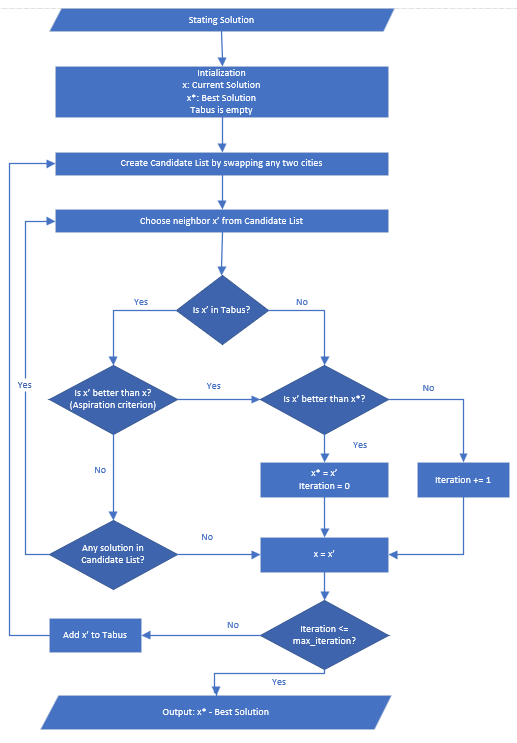
\includegraphics[width=5cm]{Tabu.png}
			\end{wrapfigure}
		Áp dụng Tabu Search vào bài toán TSP\\
		a\\
		a\\
		a\\
		a\\
		a\\
		a\\
		a\\
		a\\
		a\\
		a\\
	\end{frame}
\end{document}